\documentclass[12pt, letterpaper]{article}

% Packages
\usepackage[margin=1in]{geometry}
\usepackage{graphicx}
\usepackage{booktabs}
\usepackage{amsmath}
\usepackage{hyperref}
\usepackage{setspace}
\usepackage{parskip}
\usepackage{titlesec}
\usepackage{caption}
\usepackage{float}
\usepackage{array}
\usepackage{xcolor}

% Hyperlink styling
\hypersetup{
    colorlinks=true,
    linkcolor=black,
    urlcolor=blue,
    citecolor=black
}

% Section formatting
\titleformat{\section}{\large\bfseries}{}{0em}{}[\titlerule]
\titleformat{\subsection}{\normalsize\bfseries}{}{0em}{}

\onehalfspacing

% ────────────────────────────────────────────
\begin{document}

% Title block
\begin{center}
    {\LARGE \textbf{Student Exam Performance Analysis}} \\[0.5em]
    {\large Midterm Assessment} \\[0.5em]
    {\normalsize DATA 581 -- Data Visualization $\mid$ Gonzaga University} \\[0.3em]
    {\normalsize Harrison Christophersen $\mid$ MSDS Candidate} \\[0.3em]
    {\normalsize \today}
\end{center}

\vspace{1em}
\hrule
\vspace{1.5em}

% ────────────────────────────────────────────
\section{Executive Summary}

This report analyzes exam results for 1,000 students across three subjects --- math, reading, and writing --- to identify which background factors are most associated with performance. The goal is to give decision makers a clear picture of where additional academic support would help most.

Three patterns stand out. First, preparation pays off: students who completed the test preparation course scored approximately 7.6 points higher on average across all subjects. This is an encouraging finding because it is something a school can directly influence. Second, economic background appears to matter even more. Students on the standard lunch program scored about 8.6 points higher than those on the free or reduced lunch program --- the largest gap observed. Lunch status is commonly used as a proxy for household income, so this gap likely reflects financial circumstances at home rather than anything about student ability. The gap was widest in math. Third, reading and writing go hand in hand: a student who reads well almost always writes well, with the two scores rising and falling together almost perfectly.

\subsection*{Recommendations}
\begin{itemize}
    \item Expand access to the test preparation course, since it produced consistent gains across every subject and lies within the school's direct control.
    \item Direct additional academic support toward students on the free or reduced lunch program, where the largest performance gap appears, recognizing that some of this support may need to address circumstances outside the classroom.
    \item Treat reading and writing as a single literacy focus, since improving one tends to lift the other, making support more efficient.
\end{itemize}

% ────────────────────────────────────────────
\section{Data Overview}

The dataset contains 1,000 student records with no missing values. Each record includes three exam scores and five background attributes.

\begin{table}[H]
\centering
\caption{Dataset Variables}
\begin{tabular}{ll}
\toprule
\textbf{Variable} & \textbf{Description} \\
\midrule
gender & Female or male \\
race\_ethnicity & Anonymized group label (A through E) \\
parental\_education & Highest education level of a parent \\
lunch & Standard or free/reduced (proxy for household income) \\
test\_prep & Completed or none (proxy for study habits) \\
math score & Exam result, 0--100 \\
reading score & Exam result, 0--100 \\
writing score & Exam result, 0--100 \\
average\_score & Mean of math, reading, and writing (derived) \\
\bottomrule
\end{tabular}
\end{table}

% ────────────────────────────────────────────
\section{Summary Statistics}

Average scores across all students sit in the high 60s. Medians are nearly identical to means in every subject, indicating roughly symmetric distributions rather than skewed ones. Writing and math show the widest spread, while the combined average is the most stable --- averaging three subjects smooths out individual variation.

\begin{table}[H]
\centering
\caption{Descriptive Statistics by Subject}
\begin{tabular}{lcccc}
\toprule
\textbf{Subject} & \textbf{Mean} & \textbf{Median} & \textbf{Std Dev} & \textbf{Variance} \\
\midrule
Math          & 66.09 & 66.0 & 15.16 & 229.92 \\
Reading       & 69.17 & 70.0 & 14.60 & 213.17 \\
Writing       & 68.05 & 69.0 & 15.20 & 230.91 \\
Average Score & 67.77 & 68.3 & 14.26 & 203.27 \\
\bottomrule
\end{tabular}
\end{table}

% ────────────────────────────────────────────
\section{Exploratory Data Analysis}

\subsection{Chart 1: Average Score by Test Preparation}

Students who completed the test preparation course averaged 72.7, compared to 65.0 for those who did not --- a gap of roughly 7.6 points. The gain holds across every subject and is largest in writing. The y-axis begins at zero so bar heights represent scores proportionally.

\begin{figure}[H]
    \centering
    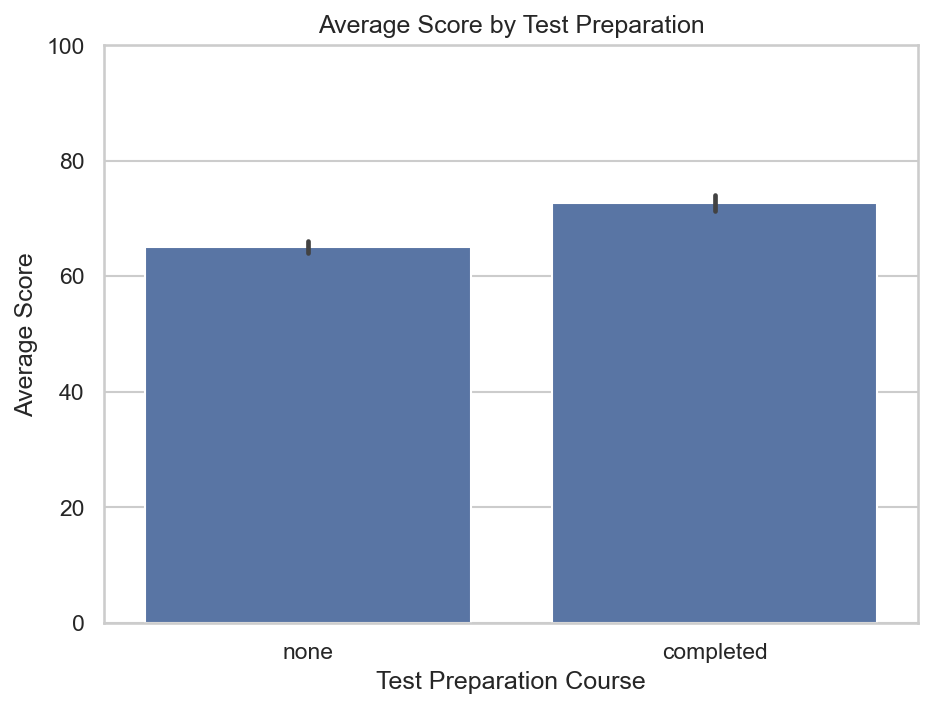
\includegraphics[width=0.7\textwidth]{chart1_test_prep.png}
    \caption{Average score by test preparation course completion.}
\end{figure}

\subsection{Chart 2: Distribution of Average Scores}

The distribution of average scores is roughly bell-shaped and centered near 68, with most students falling between approximately 55 and 80. A thin left tail identifies a small number of low performers --- the group where targeted intervention would matter most.

\begin{figure}[H]
    \centering
    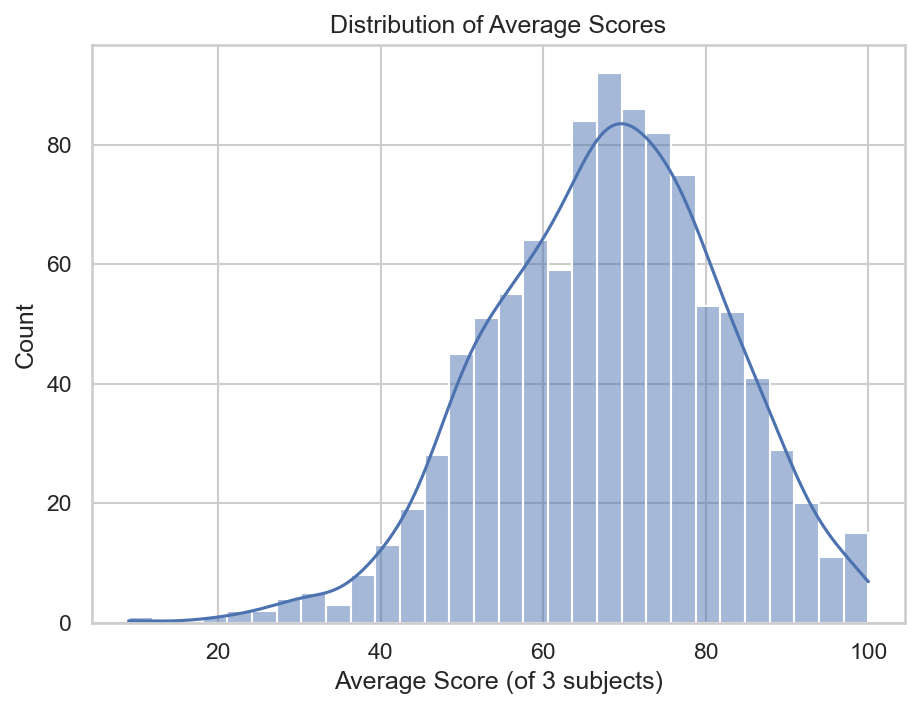
\includegraphics[width=0.7\textwidth]{chart2_distribution.png}
    \caption{Distribution of average scores across 1,000 students with KDE overlay.}
\end{figure}

\subsection{Chart 3: Reading vs.\ Writing Score Relationship}

Reading and writing scores are very strongly correlated ($r = 0.955$), meaning a student who performs well in one nearly always performs well in the other. Math is positively correlated with both ($r \approx 0.80$) but is somewhat more independent, reflecting its distinct skill set.

\begin{figure}[H]
    \centering
    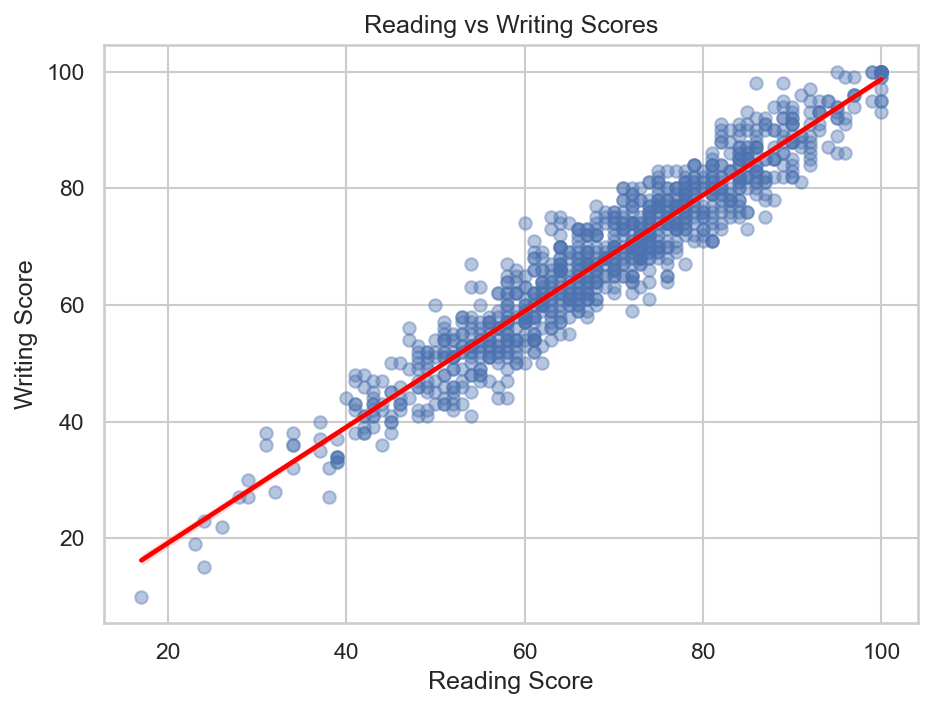
\includegraphics[width=0.7\textwidth]{chart3_reading_writing.png}
    \caption{Scatter plot of reading vs.\ writing scores with regression line.}
\end{figure}

\begin{table}[H]
\centering
\caption{Correlation Matrix}
\begin{tabular}{lccc}
\toprule
 & \textbf{Math} & \textbf{Reading} & \textbf{Writing} \\
\midrule
Math    & 1.000 & 0.818 & 0.803 \\
Reading & 0.818 & 1.000 & 0.955 \\
Writing & 0.803 & 0.955 & 1.000 \\
\bottomrule
\end{tabular}
\end{table}

\subsection{Chart 4: Average Score by Lunch Program}

Students on the standard lunch program averaged 70.8, compared to 62.2 for those on free or reduced lunch --- a gap of 8.6 points, the largest of any factor examined. The gap is widest in math at approximately 11 points. Because lunch status serves as a proxy for economic background, this finding points to the need for support that extends beyond the classroom.

\begin{figure}[H]
    \centering
    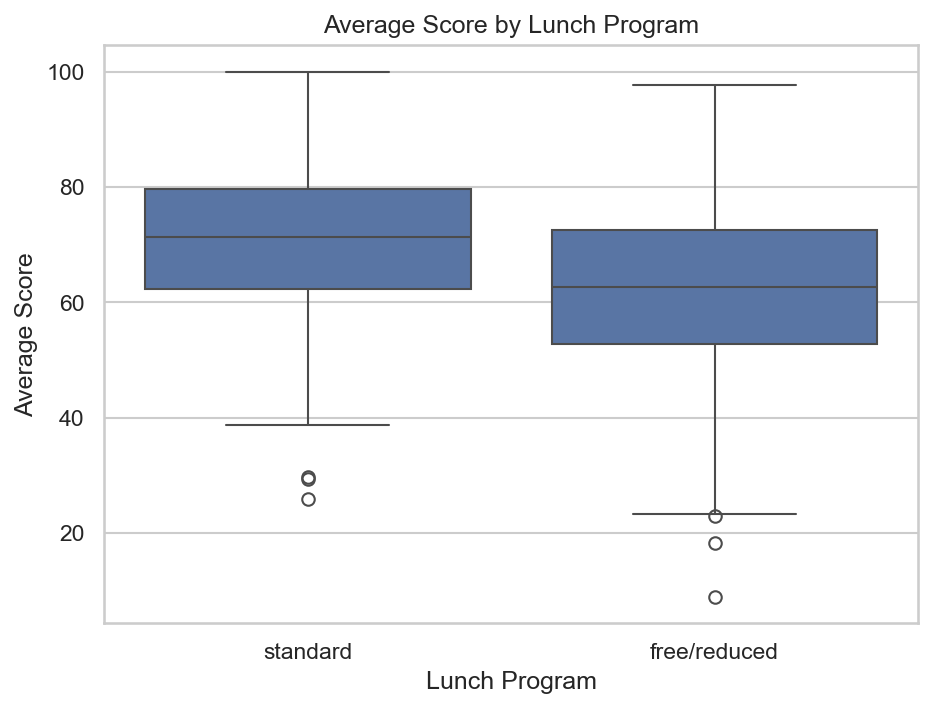
\includegraphics[width=0.7\textwidth]{chart4_lunch.png}
    \caption{Boxplot of average scores by lunch program status.}
\end{figure}

% ────────────────────────────────────────────
\section{Visualization Critique}

A deliberately misleading bar chart was constructed and then redesigned to illustrate common data visualization errors.

\subsection*{Problems Identified}
\begin{itemize}
    \item \textbf{Truncated y-axis.} Starting the axis at 94 instead of 0 makes values differing by roughly one percent (95 to 98) appear dramatically different. The tallest bar looks several times larger than the shortest when all four values are nearly identical.
    \item \textbf{Editorializing title.} The title ``AMAZING GROWTH!!!'' announces a conclusion the data does not support and adds visual emphasis with no analytical purpose.
    \item \textbf{Arbitrary color coding.} Four neon colors (red, lime, cyan, magenta) carry no meaning since the categories are not ranked or grouped.
    \item \textbf{Visual clutter.} Thick dashed gridlines, oversized fonts, and 75-degree rotated labels add noise without aiding interpretation.
\end{itemize}

\subsection*{Redesign Principles Applied}
The corrected chart starts the y-axis at zero so bar heights are proportional to their values, uses a single muted color (steelblue) since categories require no color distinction, replaces the title with a neutral description, and removes unnecessary gridlines and rotated labels.

% ────────────────────────────────────────────
\section{Ethics Reflection}

Visualizations can mislead even without intent to deceive. The most common mechanism is axis manipulation --- starting a bar chart above zero makes small differences appear dramatic. Aggregation introduces another quiet source of error: combining groups into a single average can conceal important subgroup patterns, and a trend that holds overall can even reverse within a subgroup (Simpson's Paradox).

Color choices carry implicit meaning that may not reflect the data: red signals danger, and common red-green palettes exclude colorblind readers. Omitting sample sizes or uncertainty intervals makes fragile results appear solid. Placing a strong title next to a correlation nudges viewers toward assuming causation.

These risks place a clear responsibility on analysts. Encoding data honestly means using proportional baselines so visual size matches actual magnitude. Providing context means stating what a variable actually measures --- in this project, lunch status is a proxy for income, not a judgment about a student, and saying so plainly matters. Separating evidence from recommendation means labeling associations as associations rather than dressing them up as proof. The underlying principle is straightforward: since the audience usually cannot inspect the data or the code behind a chart, the analyst's job is to make the honest reading the easiest one to reach.

% ────────────────────────────────────────────
\section{Conclusion}

Two factors stand out as most associated with student performance: lunch program status (8.6-point gap, largest observed) and test preparation course completion (7.6-point gap, most actionable). The near-perfect correlation between reading and writing ($r = 0.955$) suggests these skills share a common literacy foundation and can be developed together efficiently.

Three actions follow from the analysis: expand the test preparation course, focus additional resources on students in the free or reduced lunch program, and treat reading and writing as a unified literacy effort. These recommendations are informed starting points rather than proven causal claims --- the data is observational, and unmeasured factors including prior achievement, school quality, and home environment may contribute to the patterns observed.

% ────────────────────────────────────────────
\section*{Appendix: Key Findings Summary}

\begin{table}[H]
\centering
\caption{Summary of Key Performance Gaps}
\begin{tabular}{lcc}
\toprule
\textbf{Factor} & \textbf{Gap (avg score)} & \textbf{Largest in} \\
\midrule
Test preparation (completed vs.\ none) & 7.6 pts & Writing \\
Lunch program (standard vs.\ free/reduced) & 8.6 pts & Math \\
Gender (female vs.\ male in reading) & $\sim$5 pts & Reading/Writing \\
\bottomrule
\end{tabular}
\end{table}

\vspace{2em}
\noindent\textit{Dataset source: \href{https://www.kaggle.com/datasets/spscientist/students-performance-in-exams}{Students Performance in Exams}, Kaggle.}

\end{document}
